\documentclass[12pt]{report}
\usepackage[utf8]{inputenc}
\usepackage{amsmath,mathpazo,siunitx,xparse,tikz,enumitem,fancyhdr,pgfplots}
\usepackage{geometry}[1in]
\usepackage[document]{ragged2e}
\usepackage{tabularx}
\usepackage{tabulary}
\usepackage{pgfplotstable}
\usepackage{longtable}
\usepackage{booktabs}
\usepackage{xtab}
\usepackage{paracol}
\usepackage{array}
\usepackage{multicol}
\usepackage{paracol}
\usepackage{float}
\usepackage{mathtools}
\usetikzlibrary{patterns}

\newcommand{\me}{\mathrm{e}}

\makeatletter
\newcommand{\pgfplotsdrawaxis}{\pgfplots@draw@axis}
\makeatother
%%Needed to properly display graphs
\pgfplotsset{only axis on top/.style={axis on top=false, after end axis/.code={
             \pgfplotsset{axis line style=opaque, ticklabel style=opaque, tick style=opaque,
                          grid=none}\pgfplotsdrawaxis}},compat=1.9,width=5.5in}
%\pgfplotsset{width=10cm,compat=1.9}

\pagestyle{fancy}
\fancyhf{}
\lhead{Steven Glasford}
\chead{Homework 4}
\rhead{Page \thepage}

\title{Homework 4}
\author{Steven Glasford}
\date{\parbox{\linewidth}{\centering%
    %%Adds the last compiled date
    \today\endgraf\medskip
    Math-451-M001}}

%%Creates a new symbol for plus and minus together
\newcommand{\rpm}{\sbox0{$1$}\sbox2{$\scriptstyle\pm$}
  \raise\dimexpr(\ht0-\ht2)/2\relax\box2 }

%%Creates a nice format for displaying the steps taken  
\newlist{steps}{enumerate}{1}
\setlist[steps, 1]{label = Step \arabic*:}

\ExplSyntaxOn
%%new command to round numbers
\newcommand*{\prlen}[1]{%
   % round to 1 digit:
    \pgfmathparse{round(10)/10.0}%
    %\pgfkeys{/pgf/number format/precision=1}
    %\pgfmathresult
    \pgfmathprintnumber[fixed, precision=2]{\pgfmathresult}
}
\ExplSyntaxOff

\newcommand{\drawge}{-- (rel axis cs:1,0) -- (rel axis cs:1,1) -- (rel axis cs:0,1) \closedcycle}
\newcommand{\drawle}{-- (rel axis cs:1,1) -- (rel axis cs:1,0) -- (rel axis cs:0,0) \closedcycle}


\begin{document}
%% adds the title to the document
\maketitle
%% adds the table of contents to the document
\tableofcontents


%%%%%%%%%%%%%%%%%%%%%%%%%%%%%%%%%%%%%%%%%%%%%%%%%%%%%%%%%%%%%%%%%%%%%%%%%
%Question 10 from chapter 5
%%%%%%%%%%%%%%%%%%%%%%%%%%%%%%%%%%%%%%%%%%%%%%%%%%%%%%%%%%%%%%%%%%%%%%%%%

\chapter{RLC Circuit Problem}

\section{Problem Statement}

%Consider the electrical circuit diagrammed in Figure 5.6. The circuit consists of a capacitor, a resistor, and an inductor in a simple closed loop. The effect of each component of the circuit of is measured in terms of the relationship between current and voltage on that branch of the loop. An idealized physical model gives the relations 

%\begin{align}
%    C\dfrac{dv_C}{dt} &= i_C \label{capacitor} \\
%    v_R &= f(i_R) \label{resisotr} \\ 
%    L\dfrac{di_L}{dt} &= v_L \label{inductor}
%\end{align}

%where equation \ref{capacitor} refers to the capacitor, \ref{resisotr} refers to the resistor and \ref{inductor} refers to the inductor.
\emph{This problem is number 10 from Chapter 5 of the book.} 

Reconsider the RLC circuit of Example 5.3, but now suppose that the capacitance $C=1/5$.
\begin{enumerate}[label=(\alph*),ref=(\alph*)]
    \item\label{RLC:A} Sketch the vector field for this model.
    \item\label{RLC:B} Use the eigenvalue method to test the stability of the equilibrium at the origin.
    \item\label{RLC:C} Determine the linear system that approximates the behavior of the original dynamical system in the neighborhood of the origin. Write the general solution to this linear system, and sketch the linear phase portrait.
    \item\label{RLC:D} Sketch the complete phase portrait for this model, using the results of parts \ref{RLC:A} and \ref{RLC:C}. How does the behavior of the RLC circuit change when the capacitance $C$ is lowered? 
\end{enumerate}

This problem will heavily refer to Example 5.3 of the book.

\section{Vector Field}

In Example 5.3 several equations are given with variable $C$, so replacing $C$ with 1/5 in equations 5.20

\begin{align}
    x'_1 &= -x^3_1-4x_1-x_2 \label{RLC:x1} \\
    x'_2 &= 5x_1 \label{RLC:x2}
\end{align}

and for equation 5.21 we get 

\begin{align}
    f_1(x_1,x_2) &= -x_1^3-4x_1-x_2 \label{RLC:f1}\\
    f_2(x_1,x_2) &= 5x_1 \label{RLC:f2}
\end{align}

\begin{figure}[h]
    \centering
    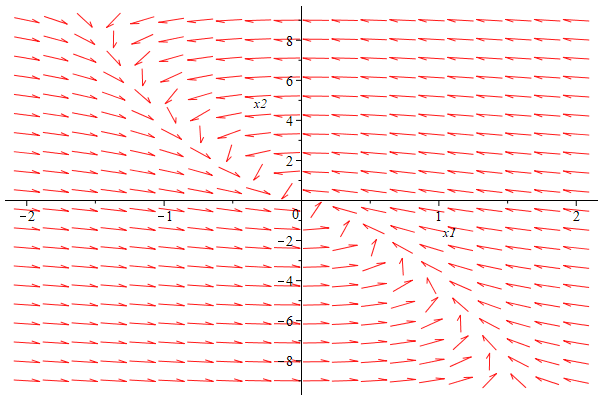
\includegraphics[width=5in]{vector.png}
    \caption{The vector field using equations \ref{RLC:x1} and \ref{RLC:x2}}
    \label{fig:vector}
\end{figure}

\section{Testing Stability using the Eigenvalue method}

In order to do the eigenvalue method we must first find the Jacobian matrix and then find the values from there, luckily however the book has already done the calculation to determine the eigenvalues which are: $$\lambda = -2 \pm \sqrt{4-\dfrac{1}{C}}$$

so plugging in $1/5$ for $C$ we get

\begin{align}
    -\lambda &= -2 \pm i \label{RLC:eigenvalues}
\end{align}

The negative component of $\lambda$ implies that the function is stable and the imaginary component implies that it is not asymptotically stable instead it has spiral stability.

\section{General Solution}
Next we need to find a linear system to approximate the solution the following function also comes from Example 5.3 in the book:

\begin{center}
    \begin{pmatrix}
        $\lambda + 4$ & $1$ \\
        $-5$ & $\lambda$
    \end{pmatrix}
    \begin{pmatrix}
        x_1\\
        x_2
    \end{pmatrix}
    $=$
    \begin{pmatrix}
        0\\
        0
    \end{pmatrix}
\end{center}

replacing lambda and using maple to find solve $\vec{X}$ we get eigenvectors of 
\begin{center}
    $k = $ \begin{bmatrix}
    -2\pm i\\5
    \end{bmatrix}
\end{center}

next we plug this information into an approximate general solution for the linear system similar to the solution of equation 5.19 in example 5.3.

\begin{center}
   
    $\begin{pmatrix}
        x_1\\x_2
    \end{pmatrix}
    = c_1\begin{pmatrix}
        -2+i\\5
    \end{pmatrix}e^{(-2+i)t}+c_2 \begin{pmatrix}
        -2-i\\5    
    \end{pmatrix}e^{(-2-i)t}$
    
\end{center}

which can be reduced using Euler's identity to an equation without imaginary numbers as:

$$\vec{X} = c_1e^{-2t} \left(\begin{bmatrix}
-2\\5
\end{bmatrix}cos(t)-\begin{bmatrix}
-2\\5
\end{bmatrix}sin(t)\right)+c_2e^{-2t} \left(\begin{bmatrix}
-2\\5
\end{bmatrix}sin(t)+\begin{bmatrix}
-2\\5
\end{bmatrix}cos(t)\right)$$

\newpage

\section{Complete Phase Portrait}
\begin{figure}[h]
    \centering
    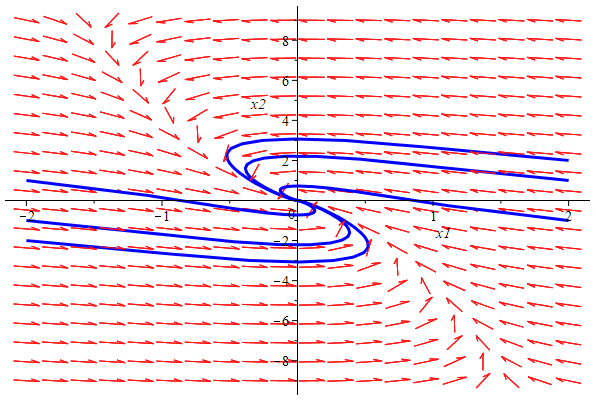
\includegraphics[width=5in]{complete.png}
    \caption{The complete phase portrait of the RLC problem}
    \label{fig:complete}
\end{figure}

\newpage

\section{Further remarks}
The behavior of the RLC circuit changes when the capacitance is lowered the swirls as seen in figure \ref{fig:complete} get tighter. Figure \ref{fig:complete1} is when the capacitance equal to 1/7, and notice how the swirls are tighter than in \ref{fig:complete}.

\begin{figure}[h]
    \centering
    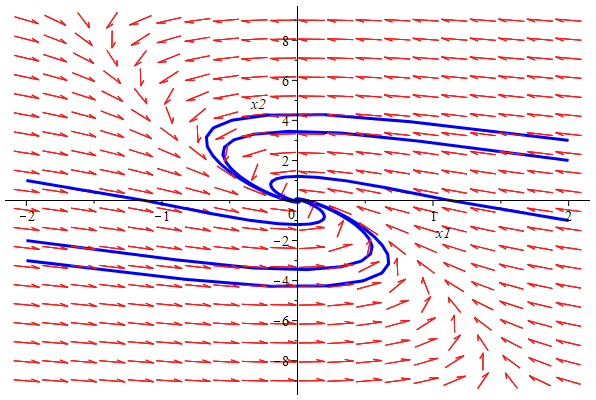
\includegraphics[width=5in]{complete1.png}
    \caption{The complete phase portrait with $C=1/7$}
    \label{fig:complete1}
\end{figure}

\chapter{Space Docking}

\secion{Problem Statement}

\begin{flushleft} 
Reconsider the space docking problem of Example 5.2, but now approximate the discrete time dynamical system 
\end{flushleft}
$$\Delta x_{1} = -kwx_{1} - kcx_{2}$$
$$\Delta x_{1} - x_{2}$$
\begin{flushleft} 
by its continuous time analogue
\end{flushleft} 
$$\dfrac{dx_{1}}{dt} = -kwx_{1} - kcx_{2}$$
$$\dfrac{dx_{2}}{dt} = x_{1} - x_{2}$$
\begin{enumerate}[label=(\alph*),ref=(\alph*)]
\item Show that the continuous time model has a stable equilibrium at (0,0). Assume $w = 10, c = 5, k = 0.02$
\item Solve the continuous model using the method of eigenvalues and eigenvectors
\item Draw the complete phase portrait for this model 
\item Comment on any differences between the behavior of the discrete and continuous model 
\end{enumerate} 

\section{Solving the Model}
\subsection{Variables \& Assumptions}
\begin{flushleft}
Given the values of $w, c,$ and $k$ we get the following continous model 
\end{flushleft} 
$$\dfrac{dx_{1}}{dt} = -0.2x_{1} - 0.1x_{2}$$
$$\dfrac{dx_{2}}{dt} = x_{1} - x_{2}$$
\begin{flushleft} 
Which we will use as the basis of our problem
\end{flushleft} 
%%%%%%%%%%%%%%%%%%%%%%%%%%%%%%%%%%%%%%%%%%%%%%%%%%%%%%%%%%%%%%%%%%%%%%%%%%%%%%%%%%%%%%%%%%%
\section{Solving the Model}
\subsection{Variables \& Assumptions}
\begin{flushleft}
Given the values of $w, c,$ and $k$ we get the following continuous model 
\end{flushleft} 
$$\dfrac{dx_{1}}{dt} = -0.2x_{1} - 0.1x_{2}$$
$$\dfrac{dx_{2}}{dt} = x_{1} - x_{2}$$
\begin{flushleft} 
Which we will use as the basis of our problem
\end{flushleft} 
\subsection{Equilibrium}
\begin{flushleft} 
We want to show that $(0,0)$ is a point of stability and equilibrium for our system. This is done by finding where our two equations equal to zero. then, we plot them and where they intersect is a point of equilibrium. 
\end{flushleft}
$$f1: x_{2} = \dfrac{-0.2x_{1}}{0.1}$$

$$f2: x_{2} = x_{1}$$
\begin{flushleft} 
When we plot these two graphs $f1$ and $f2$, as seen down below, we can see that they intersect at $(0,0)$, proving that there is equilibrium at this point. 
\end{flushleft}

\begin{center} 
\begin{tikzpicture}
\begin{axis}
[
    axis lines = left,
    xlabel = $x_{1}$,
    ylabel = $x_{2}$,
    legend pos = outer north east, 
]
%Graph 1
\addplot
 [
    domain=-2:2, 
    samples=100, 
    color=red,
    ]
{(-0.2*x)/0.1};
\addlegendentry{$f1$} 
%Graph 2
\addplot
 [
    domain=-2:2, 
    samples=100, 
    color=green,
    ]
{x};
\addlegendentry{$f2$} 
\end{axis}
\end{tikzpicture}
\end{center}

\subsection{Eigenvalue and Eigenvector Method}
\begin{flushleft}
To solve our system using the method of eigenvalues and eigenvectors, we need it in a matrix that has the following form
\end{flushleft} 
\[ \left( \begin{array}{ccc}
\dfrac{\partial f1}{x_{1}} & \dfrac{\partial f1}{x_{2}}\\
\dfrac{\partial f2}{x_{1}} & \dfrac{\partial f2}{x_{2}} \end{array} \right)\] 
\begin{flushleft}
When we go this and evaluate it at the point $(0,0)$ we obtain the following 
\end{flushleft} 
\[ \left( \begin{array}{ccc}
-0.2 & -0.1 \\
1 & 1 \end{array} \right)\] 
\begin{flushleft} 
Finding the eigenvalue we get a characteristic equation of 
\end{flushleft} 
$$ \lambda^{2} - 0.8 \lambda - 0.1$$ 
\begin{flushleft}
And solving for the eigenvalue we get eigenvalues of 
\end{flushleft} 
$$\lambda_{1} = \dfrac{4+\sqrt{26}}{10}, \lambda_{2} = \dfrac{4-\sqrt{26}}{10}$$
\begin{flushleft} 
Their perspective eigenvectors would be the following
\end{flushleft} 
\[ \left( \begin{array}{c}
-0.901 \\
1 \end{array} \right)\] 

 \[ \left( \begin{array}{c}
\dfrac{-6+\sqrt{26}}{10} \\
1 \end{array} \right)\] 

\begin{flushleft} 
With this, we can see that our general solution using the Eigenvalue and Eigenvector method is
\end{flushleft} 
$$x_{1}(t) = c_{1} * -0.901e^{ \dfrac{4+\sqrt{26}}{10}} +c_{2}*\dfrac{-6+\sqrt{26}}{10}e^{ \dfrac{4-\sqrt{26}}{10}}$$

$$ x_{2}(t) = c_{1}e^{ \dfrac{4+\sqrt{26}}{10}} +c_{2}e^{ \dfrac{4-\sqrt{26}}{10}}$$
\begin{flushleft} 
This is the general solution to our system using the eigenvalue and eigenvector method
\end{flushleft} 
%%%%%%%%%%%%%%%%%%%%%%%%%%%%%%%%%%%%%%%%%%%%%%%%%%%%%%%%%%%%%%%%%%%%%%%%%%%%%%%%%%%%%%%%%%%
\subsection{Phase Portrait}
\begin{flushleft} 
Now that we have the general solution to our system, we can choose a few values for $c_{1}$ and $c_{2}$ to plot the parametric graph. We superimpose a graph of the linear vector field in order to indicate the orientation of the solution curves. The arrows indicate the direction of the flow. This can be seen down below in figure 1.1. We can see that the vector field sinks into our point of equilibrium at $(0,0)$.
\end{flushleft} 
\begin{figure}[h]
    \centering
    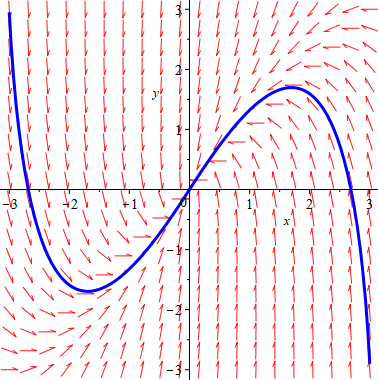
\includegraphics[width=3in]{vectorgraph.png}
    \caption{Phase Portrait}
    \label{fig:vector}
\end{figure}
%%%%%%%%%%%%%%%%%%%%%%%%%%%%%%%%%%%%%%%%%%%%%%%%%%%%%%%%%%%%%%%%%%%%%%%%%%%%%%%%%%%%%%%%%%%
\subsection{Discrete vs Continuous Models} 
\begin{flushleft}
In a discrete time model, the values of variables are remain unchanged throughout each non-zero region of time while in the continuous model that we did in the problem, the variables have a  particular value for a region between two points. Hence, why when for the discrete time $x(t)$ approaches $(0,0)$ for any initial condition. 
\end{flushleft} 

\end{document}